\newpage
\section{Практическое применение обфускатора}

\subsection{Исходный код}

Для примера возьмём программу на языке C++ из первой лабораторной работы (листинг 1).

\lstinputlisting[language=C++, caption={Исходный код программы до обфускации (src/obfuscation/main.cpp)}]
{../../src/obfuscation/main.cpp}

\subsection{Открытый обфускатор из стека LLVM}

Low Level Virtual Machine (LLVM) -- универсальная система анализа, трансформации и оптимизации программ, реализующая виртуальную машину с RISC-подобными инструкциями. Может использоваться как оптимизирующий компилятор этого байт-кода в машинный код для различных архитектур, либо для его интерпретации и JIT-компиляции (для некоторых платформ).

Расширение obfuscator-llvm позволяет проводить обфускацию кода из отдельной сборки clang. Для этого нужно скачать исходный коды из git-репозитория разработчиков и собрать их на своей машине.

В этом обфускаторе реализована замена инструкций и уплотнение графа исполнения, только не для машинного кода x86/x86-64, а для промежуточного представления LLVM-IR. Он превращает скомпилированную программу в набор символов, который практически бесполезно изучать в дизассемблере.

\begin{Verbatim}[frame=single]
$ git clone -b llvm-3.6.1 https://github.com/obfuscator-llvm/obfuscator.git
$ mkdir build
$ cd build
$ cmake -DCMAKE_BUILD_TYPE:String=Release ../obfuscator/
$ make -j5
$
\end{Verbatim}

\subsection{Результат обфускации}

Обфускатор работает на уровне промежуточного представления. Для компиляции использовался обфускатор, собранный на предыдущем шаге.

\begin{Verbatim}[frame=single]
$ build/bin/clang++ main.cpp -o netmonitor -mllvm -sub -mllvm -fla -std=c++14
\end{Verbatim}

Сам граф получен путём визуализации вызовов, полученных из valgrand

\begin{Verbatim}[frame=single]
$ valgrind --tool=callgrind -v --dump-every-bb=10000000 ./netmonitor enp2s0
\end{Verbatim}

Граф без обфускации показан на рисунке 1.

\begin{figure}[htp]
\begin{center}
  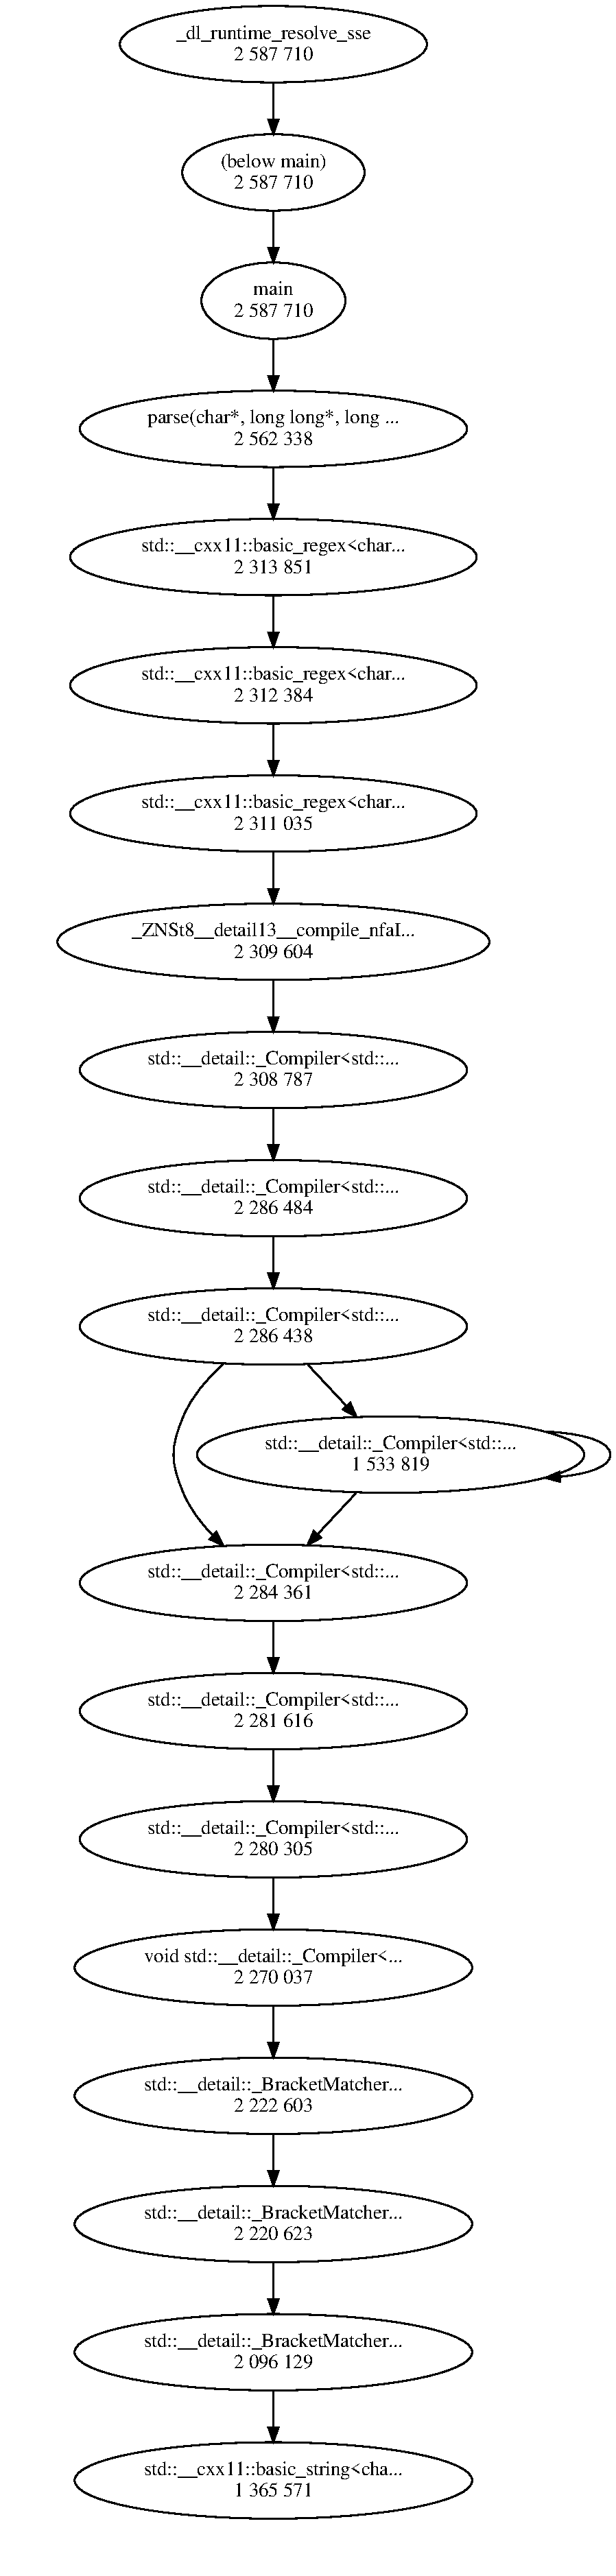
\includegraphics[width=0.33\textwidth]{res/callgraph}
  \caption{Граф вызовов до обфускации}
  \label{fig:myGraph}
\end{center}
\end{figure}

\newpage

Графов вызовов после обфускации (рисунок 2).

\begin{figure}[htp]
\begin{center}
  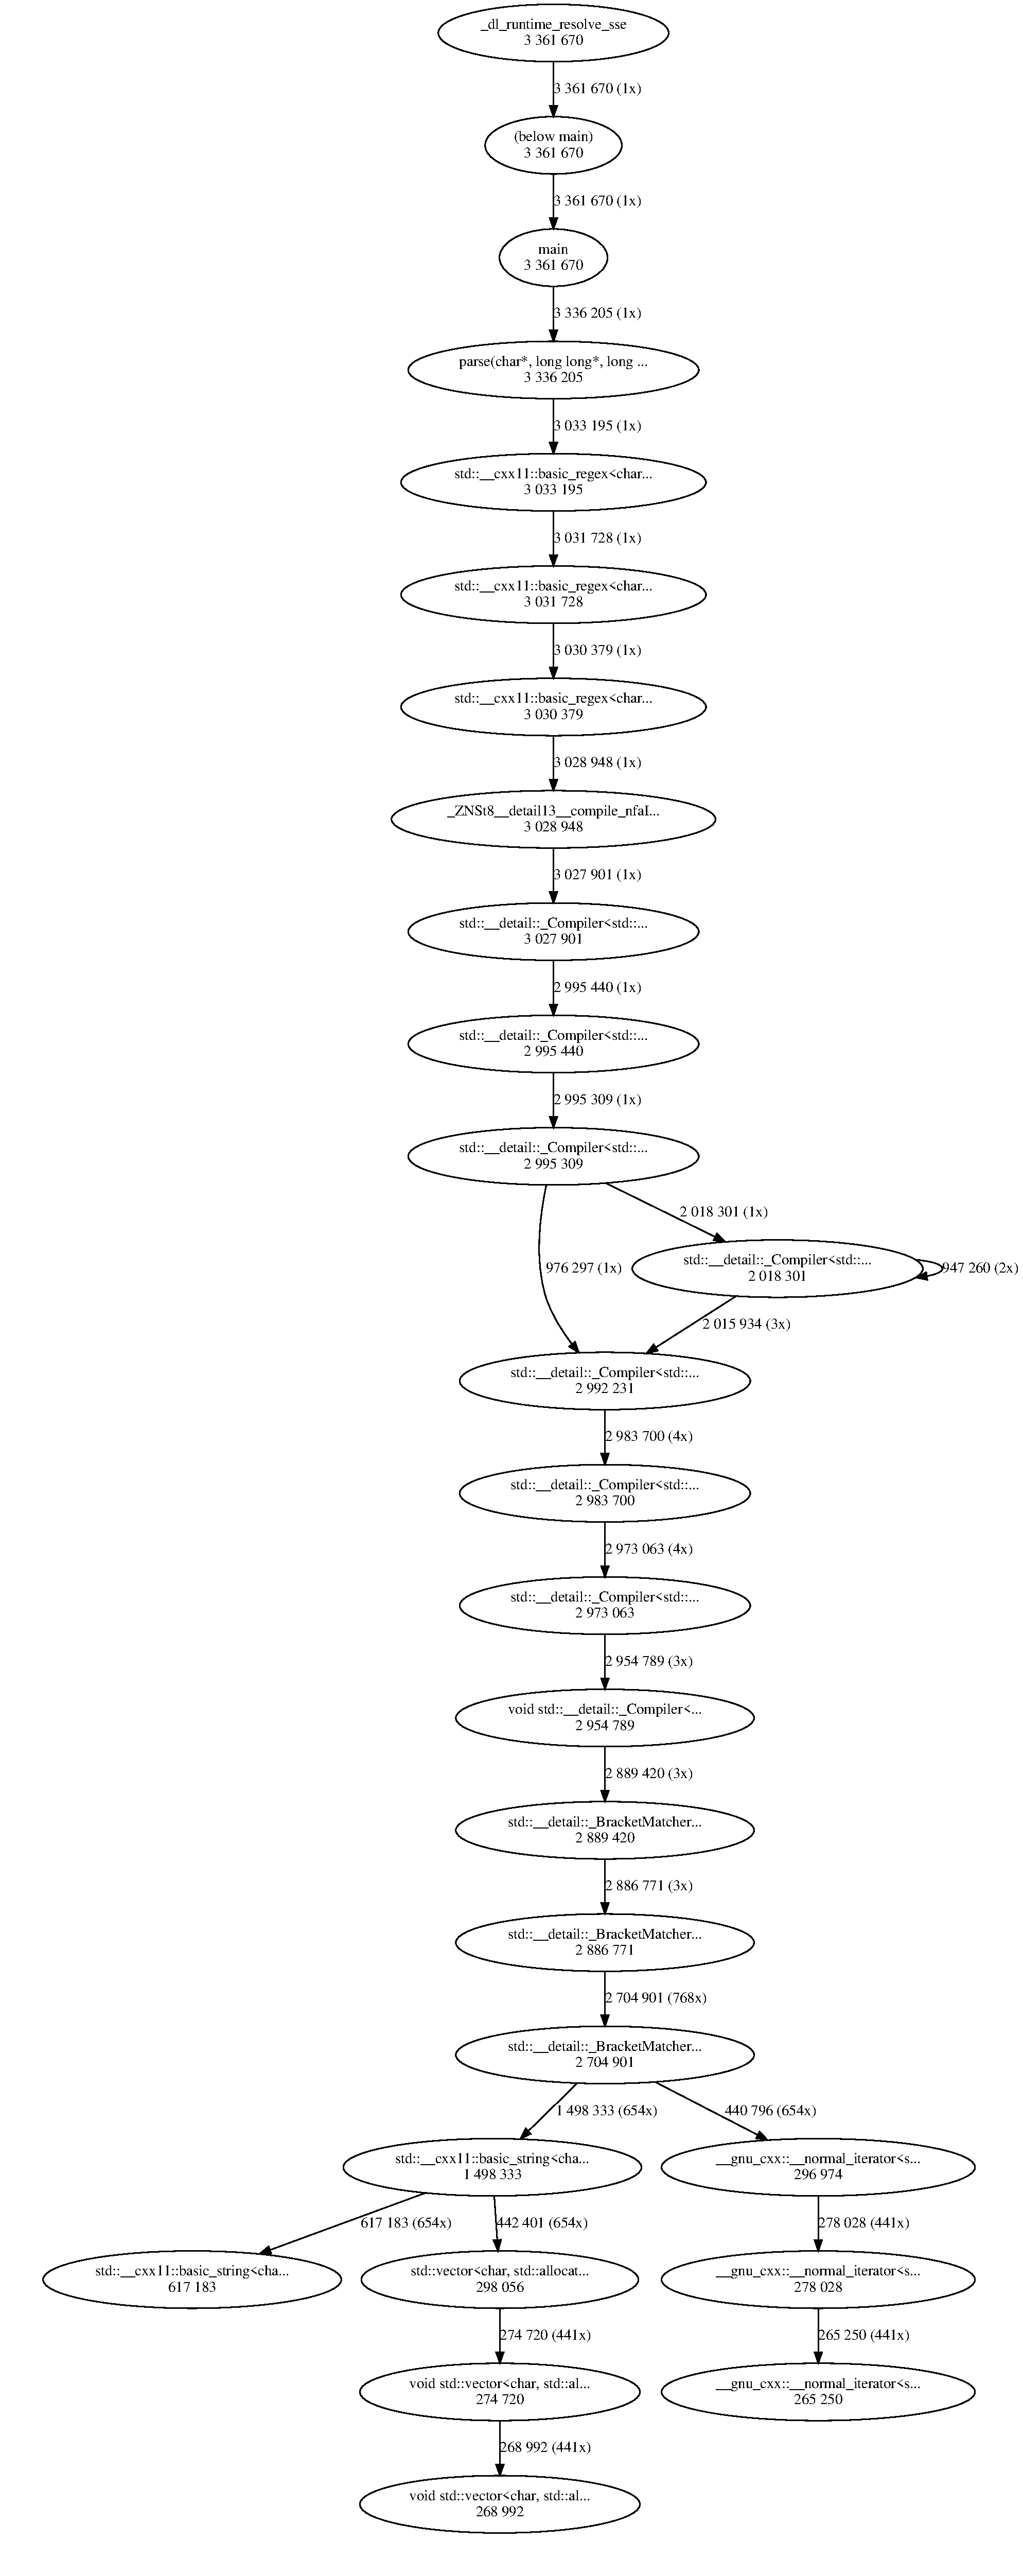
\includegraphics[width=0.41\textwidth]{res/callgraph2}
  \caption{Граф вызовов после обфускации}
  \label{fig:myGraph2}
\end{center}
\end{figure}

Как видно, графы достаточно похожи. Дело в том, что большая часть работы (парсинг строки с использованием регулярных выражений) происходит в стандартной библиотеке C++. Для повышения зашиты можно либо обфусцировать стандартную библиотеку, либо отказаться от её использования и переписать парсинг самостоятельно. Но та часть, которая отвечает за вывод информации, и которая как раз подверглась обфускации, отличается достаточно значительно.